\chapter[Dyadic Green's Function Formalism for Radiative Heat Transfer][Dyadic Green's Function Formalism for Radiative Heat Transfer]{Dyadic Green's Function Formalism for Radiative Heat Transfer} \label{ch:DGFs}
%
\section{Outline of Chapter}
%
In this chapter, I will describe a method outlined in Ref. \citenum{Narayanaswamy2013a} by which radiative heat transfer can determined between an arbitrary set of objects by using dyadic Green's functions. The method described is numerically exact, so long as the objects have isotropic linear optical properties and are isothermal and stationary. A key advantage of the method is that it relies on integration over the surfaces (not volumes) of the objects, which is both computationally inexpensive and analytically advantageous for composite bodies such as multilayered planes, cylinders, and spheres.

This chapter is structured as follows: in Section \ref{sec:Geometry} I will describe the geometric configuration for which the method is valid. Next, in Section \ref{sec:DGFs}, I will present dyadic Green's functions which can be used to solve for the electric and magnetic fields which mediate radiation heat transfer. Then, in Section \ref{sec:NFRHT}, I will show how the information described in the previous sections can be used to develop a Landauer-like formula for radiative energy transfer between arbitrary surfaces. The formalism will require knowledge of the Poynting vector and the fluctuation-dissipation theorem. The key component of the formalism is a transmissivity function which is defined in terms of the dyadic Green's functions of the system alone. Last, in Section \ref{sec:NFRHT_planeplane}, I will use the method developed to examine near-field radiative heat transfer between two homogeneous semi-infinite half-spaces.


\section{Geometry} \label{sec:Geometry}
%
A schematic of the system of objects that I will analyze is given in Fig. \ref{fig:DGF_Geometry}. $N$ objects are embedded in a free space region, labeled region $f$. Any object  $i$ ($1 \le i \le N$) is bound by a surface $S_{i}$ which separates object $i$ from region $f$. At every position on $S_{i}$, a unit normal vector, $\widehat{\boldsymbol{n}}_{i}$, can be defined which points outward into region $f$. Within surface $S_{i}$, object $i$ has well defined volume, temperature, and electromagnetic properties, which will be explored in great detail throughout this chapter. The free space region $f$ is itself bounded by surface $S_{E}$ (`E' subscript stands for environment). Though I specify a boundary to the free space region, the size of that boundary is allowed to grow such that region $f$ is effectively infinitely large. Region $f$ has a specified temperature and optical properties ($\varepsilon_{f}$ and $\mu_{f}$) which are dissipationless, i.e. $\varepsilon_{f}$, $\mu_{f}$ $\in \mathbb{R}$. Finally, $\boldsymbol{r}$ and $\widetilde{\boldsymbol{r}}$ represent position vectors which indicate various locations important to this work. They can be located anywhere within any object, or anywhere in region $f$.

\begin{figure}
\centering
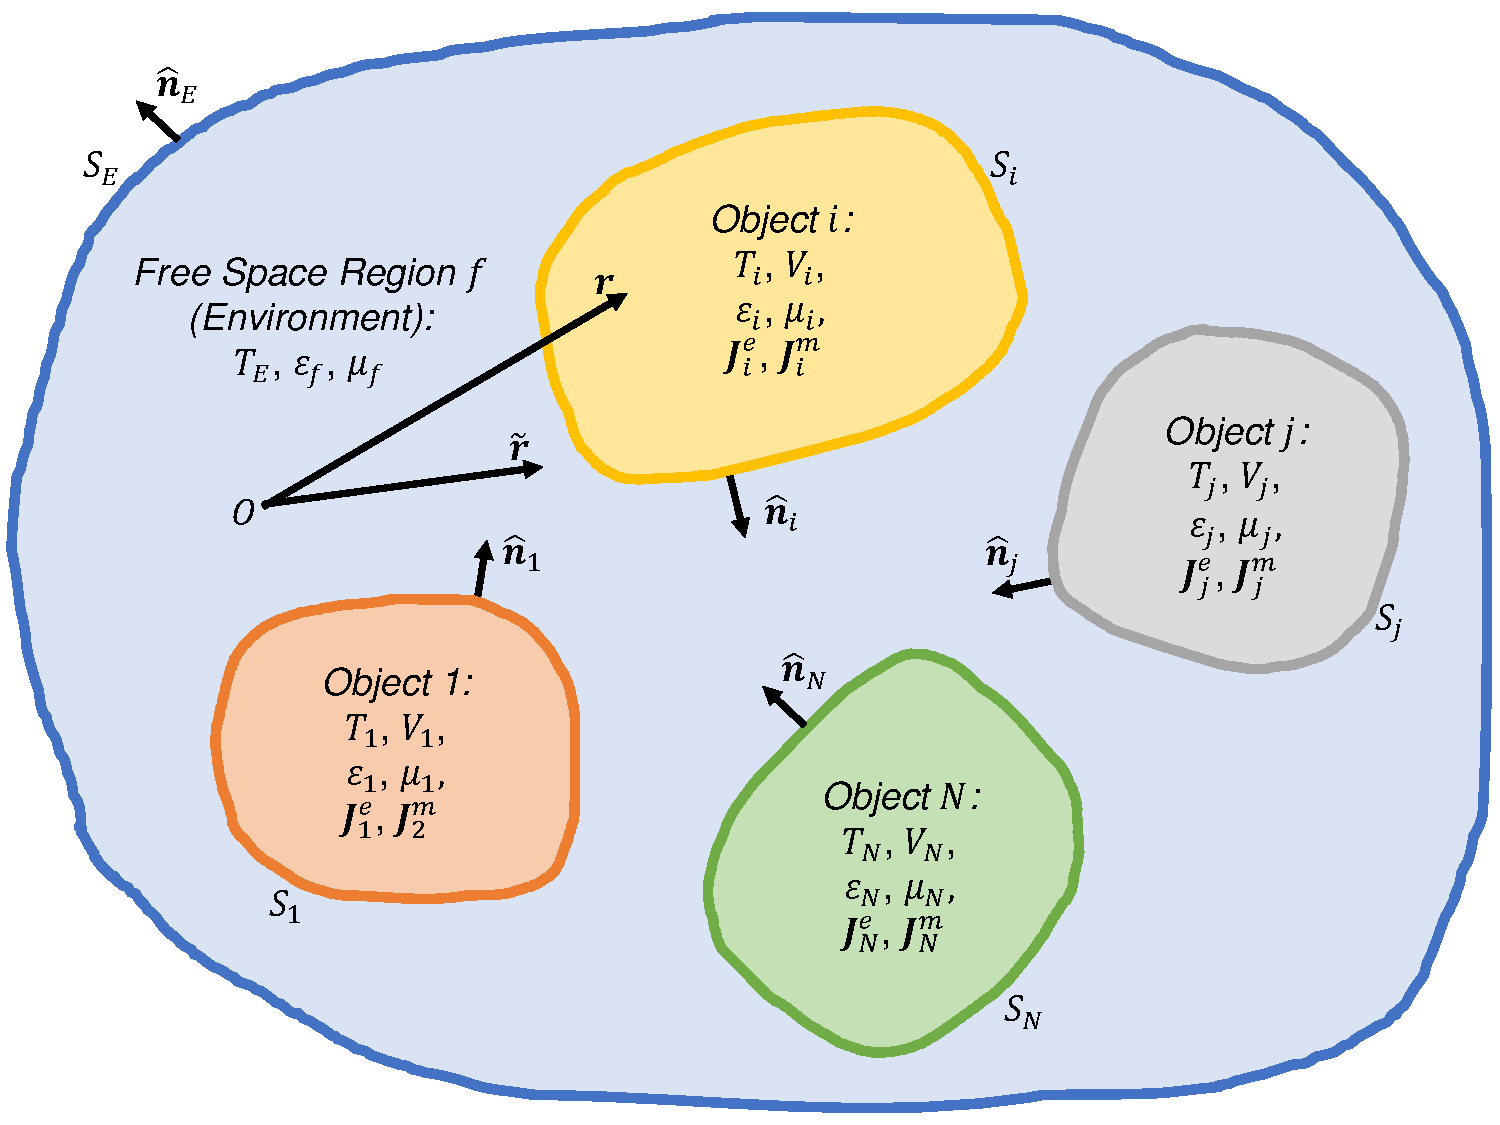
\includegraphics[width=0.8\textwidth]{./Figures/DGF_Geometry.pdf}
\caption{\label{fig:DGF_Geometry}Diagram of $N$ objects, each with its own temperature, volume, permittivity, permeability, electric free current density, and magnetic free current density. The objects are each bounded by a surface and embedded in free space region $f$, which has its own bounding surface.}
\end{figure}


\section{Dyadic Green's Functions} \label{sec:DGFs}
%
Green's functions are a powerful mathematical tool for solving boundary value problems. They represent the response of a linear differential equation at one location due to an impulse at another. A dyadic Green's function (DGF) is a Green's function which takes a vector input (for example a free current density) and produces a vector output (such as the electric field). DGFs take the form $\overline{\overline{\boldsymbol{G}}}(\boldsymbol{r}; \widetilde{\boldsymbol{r}})$ where the arguments $\boldsymbol{r}$ and $\widetilde{\boldsymbol{r}}$ are position vectors which indicate the source and response locations.

\subsection{Determining Electric and Magnetic Fields}
%
Levine and Schwinger\cite{Levine1950} first used DGFs to solve an electromagnetic boundary value problem, diffraction by an aperture in an infinite planar screen made of a conducting material. Since then, they have proven to be an invaluable tool, especially in the field of NFRHT. DGFs have been used to compute heat transfer between layered planar surfaces,\cite{Francoeur2009, Narayanaswamy2013a} spheres,\cite{Narayanaswamy2008, Sasihithlu2014, Czapla2017} and point particles,\cite{Ben-Abdallah2011, Messina2013, Asheichyk2017, Nikbakht2018} just to name a few examples.

The DGFs used to solve electromagnetism problems must satisfy the inhomogeneous vector Helmholtz equation
\begin{equation}
\boldsymbol{\nabla} \times \boldsymbol{\nabla} \times \overline{\overline{\boldsymbol{G}}}(\boldsymbol{r}; \widetilde{\boldsymbol{r}}) - k^{2}(\boldsymbol{r}) \overline{\overline{\boldsymbol{G}}}(\boldsymbol{r}; \widetilde{\boldsymbol{r}}) = \delta(\boldsymbol{r} - \widetilde{\boldsymbol{r}}) \overline{\overline{\boldsymbol{I}}}
\end{equation}

There are two variants of DGFs, electric and magnetic, which are written $\overline{\overline{\boldsymbol{G}}}_{e}(\boldsymbol{r}; \boldsymbol{\widetilde{r}})$ and $\overline{\overline{\boldsymbol{G}}}_{m}(\boldsymbol{r}; \boldsymbol{\widetilde{r}})$, respectively. The electric and magnetic variants of the DGFs can be obtained from one another by substituting $\varepsilon \leftrightarrow \mu$. Additionally, define $\overline{\overline{\boldsymbol{G}}}_{E}(\boldsymbol{r}; \boldsymbol{\widetilde{r}}) = \nabla \times \overline{\overline{\boldsymbol{G}}}_{e}(\boldsymbol{r}; \boldsymbol{\widetilde{r}})$ and $\overline{\overline{\boldsymbol{G}}}_{M}(\boldsymbol{r}; \boldsymbol{\widetilde{r}}) = \nabla \times \overline{\overline{\boldsymbol{G}}}_{m}(\boldsymbol{r}; \boldsymbol{\widetilde{r}})$, where $\nabla$ operates on functions involving $\boldsymbol{r}$ alone.

The key advantage of DGFs is that they can isolate the contributions to the electric and magnetic fields from individual sources or groups of sources, for example sources contained within a single object, like those represented in Fig. \ref{fig:DGF_Geometry}. The electric and magnetic fields themselves are superpositions of all such contributions. Define the contribution to a field $\boldsymbol{F}$ ($\boldsymbol{F}$ is $\boldsymbol{E}$ or $\boldsymbol{H}$) at location $\widetilde{\boldsymbol{r}}$ due to sources in object $i$ as $\boldsymbol{F}^{(i)}(\widetilde{\boldsymbol{r}})$. Then $\boldsymbol{F}(\widetilde{\boldsymbol{r}}) = \sum_{i=1}^{N}\boldsymbol{F}^{(i)}(\widetilde{\boldsymbol{r}})$. Obtaining $\boldsymbol{F}^{(i)}(\widetilde{\boldsymbol{r}})$ requires the inversion of Eqs. \ref{eq:MaxwellCurlElectric4} and \ref{eq:MaxwellCurlMagnetic4}. Further detail on that inversion is available in Ref. \citenum{Narayanaswamy2010}. The results of the inversion, which are presented succinctly in Ref. \citenum{Narayanaswamy2013a}, are volume integrals involving products of sources and DGFs. The volume integrals in essence calculate the net effect of all electromagnetic sources in object $i$. The volume integrals are given by
% 
\begin{subequations}
\begin{align}
\boldsymbol{E}^{(i)}(\widetilde{\boldsymbol{r}}) &= \int_{V_{i}} \left[ i \omega \mu_{0} \mu_{i} \boldsymbol{J}_{i}^{e}(\boldsymbol{r}) \cdot \overline{\overline{\boldsymbol{G}}}_{e}(\boldsymbol{r}; \widetilde{\boldsymbol{r}}) - \boldsymbol{J}_{i}^{m}(\boldsymbol{r}) \cdot \overline{\overline{\boldsymbol{G}}}_{E}(\boldsymbol{r}; \widetilde{\boldsymbol{r}}) \right] d\boldsymbol{r} \label{eq:InvertedE}
\\
\boldsymbol{H}^{(i)}(\widetilde{\boldsymbol{r}}) &= \int_{V_{i}} \left[ i \omega \varepsilon_{0} \varepsilon_{i} \boldsymbol{J}_{i}^{m}(\boldsymbol{r}) \cdot \overline{\overline{\boldsymbol{G}}}_{m}(\boldsymbol{r}; \widetilde{\boldsymbol{r}}) - \boldsymbol{J}_{i}^{e}(\boldsymbol{r}) \cdot \overline{\overline{\boldsymbol{G}}}_{M}(\boldsymbol{r}; \widetilde{\boldsymbol{r}}) \right] d\boldsymbol{r} \label{eq:InvertedH}
\end{align} \label{eq:InvertedFields}
\end{subequations}
%
where $\boldsymbol{r}$ lies within the volume of object $i$. The terms in the integrals should look familiar; they are the right hand side source terms in Eqs. \ref{eq:MaxwellCurlElectric4} and \ref{eq:MaxwellCurlMagnetic4}. 

\subsection{Boundary Conditions}
%
Solving the vector Helmholtz equation is essentially a boundary value problem, so it should come as a surprise to no one that knowledge of the boundary conditions of DGFs will prove vital. Maxwell's equations, in their integral form, guarantee continuity of the tangential components of the electric and magnetic fields across a boundary. Written in terms of DGFs, we get
%
\begin{subequations}
\begin{align}
& \widehat{\boldsymbol{n}}(\boldsymbol{r}) \times \left[\left[ \mu(\boldsymbol{r}) \overline{\overline{\boldsymbol{G}}}_{e}(\boldsymbol{r}; \widetilde{\boldsymbol{r}}) \right]\right] = 0 \\
& \widehat{\boldsymbol{n}}(\boldsymbol{r}) \times \left[\left[ \overline{\overline{\boldsymbol{G}}}_{E}(\boldsymbol{r}; \widetilde{\boldsymbol{r}}) \right]\right] = 0 \\
& \widehat{\boldsymbol{n}}(\boldsymbol{r}) \times \left[\left[ \varepsilon(\boldsymbol{r}) \overline{\overline{\boldsymbol{G}}}_{m}(\boldsymbol{r}; \widetilde{\boldsymbol{r}}) \right]\right] = 0 \\
& \widehat{\boldsymbol{n}}(\boldsymbol{r}) \times \left[\left[ \overline{\overline{\boldsymbol{G}}}_{M}(\boldsymbol{r}; \widetilde{\boldsymbol{r}}) \right]\right] = 0
\end{align} \label{eq:DGF_BCs}
\end{subequations}
%
where $\widehat{\boldsymbol{n}} \times \left[\left[ \overline{\overline{\boldsymbol{f}}} \right]\right] \equiv \widehat{\boldsymbol{n}} \times \left( \overline{\overline{\boldsymbol{f}}}_{+} - \overline{\overline{\boldsymbol{f}}}_{-} \right)$ denotes a jump condition across an interface and $\widehat{\boldsymbol{n}}$ is the unit outward normal pointing to the `+' side of the interface.\cite{Ateshian2007, Satapathy2013}


\section{Radiative Heat Transfer Between Arbitrary Surfaces} \label{sec:NFRHT}
%
Now that we are able to determine electric and magnetic fields by using the DGFs of the system, in conjunction with any sources of electromagnetic waves, we can move on to computing the net radiative transfer between objects. The strategy to compute the heat transfer using Maxwell's equations is as follows: (1) Determine the Poynting vector at the surface of an object to understand the flow of electromagnetic energy into the object. (2) Determine the time-averaged behavior of electromagnetic sources using the fluctuation-dissipation theorem. (3) Combine those results with the results of the previous section to determine formulas which give the net radiative transfer.

\subsection{Poynting Vector}
%
The Poynting vector, $\boldsymbol{P}$, is defined such that its magnitude and direction hold special significance in electromagnetism; they represent the intensity and direction of flow of electromagnetic energy at a given point. Its name is almost serendipitous, since it can be said to point in the direction of the flow. But the Poynting vector is actually named after the English physicist John Henry Poynting, who first published about it in 1884.\cite{Poynting1884}

The time-averaged contribution to the Poynting vector at a position $\widetilde{\boldsymbol{r}}$ due to sources in object $i$ given by
%
\begin{align}
\boldsymbol{P}^{(i)}(\boldsymbol{\widetilde{r}}) &= \frac{1}{2\pi} \mathrm{Re} \int_{0}^{\infty} \left< \boldsymbol{E}^{(i)}(\boldsymbol{\widetilde{r}}) \times \boldsymbol{H}^{(i)*}(\boldsymbol{\widetilde{r}}) + \boldsymbol{E}^{(i)*}(\boldsymbol{\widetilde{r}}) \times \boldsymbol{H}^{(i)}(\boldsymbol{\widetilde{r}}) \right> d\omega \label{eq:PoyntingVector}
\end{align}
%
where $\left< \cdot \right>$ denotes an ensemble average and  $\left(\cdot\right)^{*}$ is the complex conjugate. Due to linearity, the same formula is true after the substitution $\boldsymbol{P}^{(i)} \rightarrow \boldsymbol{P}$, $\boldsymbol{E}^{(i)} \rightarrow \boldsymbol{E}$, and $\boldsymbol{H}^{(i)} \rightarrow \boldsymbol{H}$. As evident by the formula, $\boldsymbol{P}^{(i)}$ is related to the cross-spectral density of the components of the electric and magnetic fields and has contributions from all frequencies. It is important to note here that, despite not being written explictly, the electric and magnetic fields both vary with frequency.

If Eqs. \ref{eq:InvertedE} and \ref{eq:InvertedH} are used to determine $\boldsymbol{E}^{(i)}(\boldsymbol{\widetilde{r}})$ and $\boldsymbol{H}^{(i)}(\boldsymbol{\widetilde{r}})$, the resulting Poynting vector gives the flow of electromagnetic energy due to sources only within the volume of object $i$. This is very useful when isolating thermal radiation between pairs of objects.

From Eq. \ref{eq:PoyntingVector}, we can see that we need to evaluate products of the electric and magnetic fields. The products contain terms which are ensemble averages of the products of the free current densities, $\boldsymbol{J}_{i}^{e}$ and $\boldsymbol{J}_{i}^{m}$. In order to evaluate those terms, we must turn to the fluctuation-dissipation theorem to better understand the statistical nature of the sources of electromagnetic radiation.


\subsection{Fluctuation-Dissipation Theorem}
%
Any object at a finite temperature, even if at equilibrium, will experience random deviations from equilibrium due to its thermal energy. When these fluctuations involve charges like electrons, the acceleration of the electrons will result in the radiation of electromagnetic waves. Although the currents due to fluctuating charges will average to zero overtime, the products of currents need not also average to zero. This is where the fluctuation-dissipation theorem comes in.

The fluctuation-dissipation theorem relates the spectral density of random fluctuations of a system to the system's dissipation. Much of the preliminary work relating fluctuation and dissipation was performed by Harry Nyquist, who investigated such a relation for conductors.\cite{Nyquist1928} His work was only applicable in the low-frequency limit. The first theory to connect fluctuations out of equilibrium and dissipation in a general linear system was completed by Callen and Welton in 1951.\cite{Callen1951} In 1953, Rytov connected thermal radiation to fluctuations currents using the fluctuation-dissipation theorem.\cite{Rytov1953, Rytov1959} His work continues to motivate modern work in NFRHT, as well as work on the van der Waals and Casimir forces.\cite{Lipshitz1956, Dzyaloshinskii1961}

The spectral densities of the components of $\boldsymbol{J}_{i}^{e}(\boldsymbol{r})$ and $\boldsymbol{J}_{i}^{m}(\boldsymbol{r})$ are related by the fluctuation-dissipation theorem of the second kind \cite{Eckhardt1982} 
%
\begin{subequations} \label{eq:FlucDiss}
\begin{align}
\left< \boldsymbol{J}_{i,p}^{e}(\boldsymbol{r}) \boldsymbol{J}_{i,q}^{e*}(\widetilde{\boldsymbol{r}}) \right> &= 2 \omega \varepsilon_{0} \mathrm{Im}{\left( \varepsilon \right)} \Theta(\omega,T) \delta \! \left( \boldsymbol{r} - \boldsymbol{\widetilde{r}} \right) \delta_{pq}
\\
\left< \boldsymbol{J}_{i,p}^{m}(\boldsymbol{r}) \boldsymbol{J}_{i,q}^{m*}(\widetilde{\boldsymbol{r}}) \right> &= 2 \omega \mu_{0} \mathrm{Im}{\left( \mu \right)} \Theta(\omega,T) \delta \! \left( \boldsymbol{r} - \boldsymbol{\widetilde{r}} \right) \delta_{pq}
\\
\left< \boldsymbol{J}_{i,p}^{e}(\boldsymbol{r}) \boldsymbol{J}_{i,q}^{m*}(\widetilde{\boldsymbol{r}}) \right> &= 0
\end{align}
\end{subequations}
%
where $p,q=1,2,3$ are the Cartesian components of the current densities, $\mathrm{Im}{\left(\cdot\right)}$ denotes the imaginary component, $T$ is the thermodynamic temperature, and $\Theta(\omega, T)$ is the average energy of a harmonic oscillator of frequency $\omega$ at temperature $T$. In Eq. \ref{eq:FlucDiss}, $\boldsymbol{J}_{i}^{e}(\boldsymbol{r})$ and $\boldsymbol{J}_{i}^{m}(\boldsymbol{r})$ represent the fluctuation and $\mathrm{Im}{\left( \varepsilon \right)}$ and $\mathrm{Im}{\left( \mu \right)}$ represent the dissipation. The delta function $\delta_{pq}$ makes clear there is no coupling between charge fluctuations in orthogonal directions. The delta function $\delta(\boldsymbol{r} - \widetilde{\boldsymbol{r}})$ shows that there is no spatial correlation in currents, and is known as the local approximation. This work will assume the validity of such an approximation, though I direct authors to Ref. \citenum{Singer2015} for work on NFRHT between non-local materials with spatial dispersion.

The average energy of a harmonic oscillator is given by
%
\begin{equation}
\begin{split}
\Theta &= k_{b} T \mathcal{X} \coth{\left( \mathcal{X} \right)}
\\
&= k_{b} T \mathcal{X} \left( 1 + \frac{2}{\exp{\left( 2 \mathcal{X} \right)} - 1} \right) 
\end{split}
\end{equation}
%
where $\mathcal{X} = \hbar\omega/(2 k_{b} T)$, $\hbar$ is the reduced Planck's constant, and $k_{b}$ is Boltzmann's constant. The lone $k_{b} T \mathcal{X}$ summand in the second line corresponds to the zero point energy. Many works in NFRHT exclude the term when defining $\Theta$ because it does not contribute to the net transfer of heat, but we keep it here for completeness.


\subsection{Heat Transfer and Conductance}
%
The goal of this chapter was to write a general formula for NFRHT in a Landauer-like form, one in which the formulas for thermal transport are given in terms of modes and probabilities of transmission of energy. Now that we can compute all the necessary terms to understand the electromagnetic fields and the flow of electromagnetic energy, we can begin to address radiative transfer. The radiative transfer through surface $S_{i}$ due to sources within object $j$ is given by
%
\begin{align}
Q_{t, j \rightarrow i} &= - \oint_{S_i} \left[ \widehat{\boldsymbol{n}}_{i}(\boldsymbol{\widetilde{r}}) \cdot \boldsymbol{P}^{(j)}(\boldsymbol{\widetilde{r}}) \right] d\boldsymbol{\widetilde{r}},
\label{eq:HeatTransfer1}
\end{align}
%
where $\boldsymbol{\widetilde{r}}$ points to positions on surface $S_{i}$ and the negative sign is required because $\widehat{\boldsymbol{n}}_{i}$ is unit outward normal of the surface and we require energy flow inward. Using Eqs. \ref{eq:PoyntingVector} (Poynting vector), \ref{eq:InvertedFields} (electric and magnetic fields), and \ref{eq:FlucDiss} (fluctuation-dissipation theorem), we can evaluate Eq. \ref{eq:HeatTransfer1} and get a result in terms of only the DGFs of the system, temperatures, and optical properties. We get
%
\begin{align}
Q_{t, j \rightarrow i} &= \frac{1}{2\pi} \int_{0}^{\infty} \left[ \Theta(\omega, T_{j}) - \Theta(\omega, T_{E}) \right] \tau_{j \rightarrow i}(\omega) d\omega
\label{eq:HeatTransfer2}
\end{align}
%
where $\tau_{j \rightarrow i}(\omega)$ is a temperature-independent transmissivity function for energy transfer between objects $i$ and $j$. In some sense, it is a catch-all function for all the terms you get when you evaluate Eq. \ref{eq:HeatTransfer1}. But the function has a number of convenient features which will be discussed at length in the next subsection. The net radiative transfer from object $j$ to object $i$ is given by
%
\begin{equation}
\begin{split}
Q_{t, j \rightarrow i}^{(\mathrm{net})} &= Q_{t, j \rightarrow i} - Q_{t, i \rightarrow j} = \int_{0}^{\infty} Q_{j \rightarrow i}^{(\mathrm{net})}(\omega) d\omega
\\
&= \frac{1}{2\pi} \int_{0}^{\infty} \left[ \Theta(\omega, T_{j}) - \Theta(\omega, T_{i}) \right] \tau_{j \rightarrow i}(\omega) d\omega
\label{eq:NetHeatTransfer}
\end{split}
\end{equation}

This simplification is enabled because $\tau_{i \rightarrow j} = \tau_{j \rightarrow i}$.\cite{Narayanaswamy2013a} From Eq. \ref{eq:NetHeatTransfer}, is it clear to see $Q_{t,j \rightarrow i}^{(\mathrm{net})} = - Q_{t,i \rightarrow j}^{(\mathrm{net})}$, which fits with our expectation for radiative transfer.

An additional quantity useful to analyzing systems of objects exchanging radiation is the conductance. Conductance is the proportionality constant between $Q$ and $\Delta T$, and can be used to linearize the temperature dependence of thermal radiation when $\Delta T$ is small. Define two conductances, a spectral ($G$) and a total conductance ($G_{t}$), given by
%
\begin{align}
G_{j \rightarrow i}(\omega, T) &= \lim_{T_{j},T_{i} \rightarrow T} \frac{Q_{j \rightarrow i}^{\mathrm{(net)}}(\omega)}{T_{j}-T_{i}} =  \frac{\partial \Theta}{\partial T} \tau_{j \rightarrow i} \left( \omega \right)
\\
G_{t, j \rightarrow i}(T) &= \frac{1}{2\pi} \int_{0}^{\infty} G_{j \rightarrow i}(\omega, T) d\omega
\end{align}

Working with conductance has the advantage of reducing the number of temperatures variables to one. To calculate conductances, the temperature dependence is captured by the temperature derivative of $\Theta$
%
\begin{equation} \label{eq:TemperatureDerivative}
\begin{split}
\frac{\partial \Theta}{\partial T} &= k_{b} \mathcal{X}^{2} \csch^{2}{\left( \mathcal{X} \right)}
\\
&= k_{b} \left( 2 \mathcal{X} \right)^{2} \frac{ \exp{\left( 2 \mathcal{X} \right)} }{ \left( \exp{\left( 2 \mathcal{X} \right)} - 1 \right)^{2} }
\end{split}
\end{equation}

Spectral conductance is often expressed in different units in different papers, but changes of variable can be performed to transform between units. A definition of spectral conductance is valid so long as the integral defintion of total conductance computes to the same value, regardless of the units used. For example, in Fig. \ref{fig:ThreeSpheres_SCUFFEM} I present $\tau_{j \rightarrow i}(\lambda)$ in units of \si{\per\second \per\micro\meter}, where $\lambda = 2 \pi c / \omega$ is the vacuum wavelength and $c$ is speed of light in vacuum. This version of spectral conductance is obtained from $\tau_{j \rightarrow i}(\lambda) = c \lambda^{-2} \tau_{j \rightarrow i}(\omega)$ and the corresponding integral definition for total conductance is
%
\begin{equation} \label{eq:TotalConductance_wavelength}
\begin{split}
G_{t,j \rightarrow i}(T) &= \int_{0}^{\infty} G_{j \rightarrow i}(\lambda, T) d\lambda
\\
&= \int_{0}^{\infty} k_{b} \mathcal{X}^{2} \csch^{2}{\left( \mathcal{X} \right)} \tau_{j \rightarrow i}(\lambda) d\lambda 
\end{split}
\end{equation}


\subsection{Transmissivity Function}
%
As was stated earlier, DGFs take the form $\overline{\overline{\boldsymbol{G}}}(\boldsymbol{r}; \widetilde{\boldsymbol{r}})$ where the arguments $\boldsymbol{r}$ and $\widetilde{\boldsymbol{r}}$ are position vectors which indicate the source and response locations. Depending on which regions $\boldsymbol{r}$ and $\widetilde{\boldsymbol{r}}$ are located, both the DGFs themselves and the form of the transmissivity function must change. The transmissivity function was derived using Eq. \ref{eq:InvertedFields} (volume integration) and Eq. \ref{eq:HeatTransfer1} (surface integration). That asymmetry has a number of disadvantages, primarily that it obscures the symmetry of radiative heat transfer. Since emission and absorption of electromagnetic waves are volumetric phenomena, it might seem intuitive to expect the expression for the transmissivity function for energy transfer to contain two volume integrals, and thus to convert the surface integral to a volume integral. Double volume integral was the approach that allowed Polder and van Hove to derive their plane-plane NFRHT\cite{Polder1971} and for Narayanaswamy and Chen to derive the first sphere-sphere NFRHT result.\cite{Narayanaswamy2008} But that approach is limited because any composite bodies would require volume integration over each interior region separately. While that is not impossible, it is cumbersome.

If the volumes are isothermal, the properties of the vector Helmholtz equation allow us to convert volume integrals into surface integrals. If the volume integral is converted to a surface integral, we get the approach called the ``interior method'' by Narayanaswamy and Zheng in Ref. \citenum{Narayanaswamy2013a}. When using the interior method, though the integrations occur on the two surfaces, $\boldsymbol{r}$ and $\widetilde{\boldsymbol{r}}$ must approach the two surfaces from the insides of the objects. The transmissivity function for such a situation is given by
%
\begin{align}
\tau_{j \rightarrow i} (\omega) &= 2 \mathrm{Re} \mathrm{Tr} \oint_{S_i} d\boldsymbol{r} \oint_{S_j} d\boldsymbol{\widetilde{r}}
\left[ \!\! \begin{array}{r} \! \! \left( \frac{\omega}{c} \right)^{2} \! \! \varepsilon^{*}(\boldsymbol{r}) \mu(\boldsymbol{r}) \bigg[ \boldsymbol{\widehat{n}}_{i}(\boldsymbol{r}) \times \overline{\overline{\boldsymbol{G}}}_{e}(\boldsymbol{r}, \widetilde{\boldsymbol{r}}) \bigg] \! \cdot \! \bigg[ \boldsymbol{\widehat{n}}_{j}(\boldsymbol{\widetilde{r}}) \times \overline{\overline{\boldsymbol{G}}}_{m}^{T}(\boldsymbol{r}, \boldsymbol{\widetilde{r}}) \bigg]^{*} \\
+ \bigg[ \boldsymbol{\widehat{n}}_{i}(\boldsymbol{r}) \times \overline{\overline{\boldsymbol{G}}}_{M}(\boldsymbol{r}, \boldsymbol{\widetilde{r}}) \bigg] \! \cdot \! \bigg[ \boldsymbol{\widehat{n}}_{j}(\boldsymbol{\widetilde{r}}) \times \overline{\overline{\boldsymbol{G}}}_{E}^{T}(\boldsymbol{r}, \boldsymbol{\widetilde{r}}) \bigg]^{*}
\end{array} \!\! \right] \label{eq:Transmissivity_Interior}
\end{align}

In some ways, the double surface integral formula for the transmissivity function appears similar to the formula for a view factor \cite{Howell2011} in classical radiative transfer. The view factor, however, is a purely geometric property of just two objects, irrespective of any other objects present, whereas the DGFs contained within the transmissivity function automatically account for the effects of all objects present. Furthermore classical approaches such as thermal circuits or Gebhart factors \cite{Gebhart1961}, when using view factors in their calculations, assume objects emit diffusly with well-defined emissivities. DGF approaches, and therefore the transmissivity function, are exact in all situations where Maxwell's equations are valid, which includes objects with super-Planckian (greater than that of a blackbody) effective emissivities.

The boundary conditions given by Eq. \ref{eq:DGF_BCs} allow us to move from the interior method to an ``exterior method," one for which $\boldsymbol{r}$ and $\widetilde{\boldsymbol{r}}$ must approach the two surfaces from the outsides of the objects, in free-space region $f$. The advantage of this approach is that the same formalism can be used for homogeneous or composite objects. The transmissivity function for that case is given by
%
\begin{align}
\tau_{j \rightarrow i} (\omega) &= 2 \mathrm{Re} \mathrm{Tr} \oint_{S_i} d\boldsymbol{r} \oint_{S_j} d\boldsymbol{\widetilde{r}}
\left[ \begin{array}{r} k_{f}^{2} \bigg[ \boldsymbol{\widehat{n}}_{i}(\boldsymbol{r}) \times \overline{\overline{\boldsymbol{G}}}_{e}(\boldsymbol{r}, \widetilde{\boldsymbol{r}}) \bigg] \cdot \bigg[ \boldsymbol{\widehat{n}}_{j}(\boldsymbol{\widetilde{r}}) \times \overline{\overline{\boldsymbol{G}}}_{m}^{T}(\boldsymbol{r}, \boldsymbol{\widetilde{r}}) \bigg]^{*} \\
+ \bigg[ \boldsymbol{\widehat{n}}_{i}(\boldsymbol{r}) \times \overline{\overline{\boldsymbol{G}}}_{M}(\boldsymbol{r}, \boldsymbol{\widetilde{r}}) \bigg] \cdot \bigg[ \boldsymbol{\widehat{n}}_{j}(\boldsymbol{\widetilde{r}}) \times \overline{\overline{\boldsymbol{G}}}_{E}^{T}(\boldsymbol{r}, \boldsymbol{\widetilde{r}}) \bigg]^{*}
\end{array} \right] \label{eq:Transmissivity_Exterior}
\end{align}

At first glance, the transmissivity function for the exterior method does not appear very different than that of the interior method. The key difference between the two is that the DGFs needed to use this formalism are different than those for the interior method. The DGFs must be determined such that both of the position vector arguments are located in free space region $f$, just outside the surfaces of objects $i$ and $j$. The exterior method will be the approach favored throughout this work.


\section{Radiative Heat Transfer Between Planar Bodies} \label{sec:NFRHT_planeplane}
%
The NFRHT between two planar half-spaces has been well-studied since Polder and van Hove first published their work in 1971.\cite{Polder1971} In this section, I will present theoretical and numerical results for plane-plane NFRHT. Using the exterior method (see Ref. \citenum{Narayanaswamy2013a} for the appropriate DGFs), the transmissivity (per unit area) between two semi-infinite half-spaces is given by 
%
\begin{equation}
\frac{\tau_{1 \rightarrow 2}(\omega)}{A} = \frac{1}{2\pi} \int_{0}^{\infty} \left[ \mathcal{T}^{(s)}(k_{\rho}) + \mathcal{T}^{(p)}(k_{\rho}) \right] k_{\rho} dk_{\rho}
\end{equation}
%
where
\begin{equation}
\mathcal{T}^{(\alpha)}(k_{\rho}) = \left\{ \begin{array}{lcc}
\frac{\left( 1 - \left| \widetilde{r}_{1}^{(\alpha)} \right|^{2} \right) \left( 1 - \left| \widetilde{r}_{2}^{(\alpha)} \right|^{2} \right)}{\left| 1 - \widetilde{r}_{1}^{(\alpha)} \widetilde{r}_{2}^{(\alpha)} \exp{\left( 2ik_{z,0} l \right)} \right|^{2}} & \mathrm{if} & 0 \le k_{\rho} \le \omega/c \\
\frac{4 \mathrm{Im}\left( \widetilde{r}_{1}^{(\alpha)} \right) \mathrm{Im}\left( \widetilde{r}_{2}^{(\alpha)} \right) \exp{\left( 2ik_{z,0} l \right)}}{\left| 1 - \widetilde{r}_{1}^{(\alpha)} \widetilde{r}_{2}^{(\alpha)} \exp{\left( 2ik_{z,0} l \right)} \right|^{2}} & \mathrm{if} & \omega/c < k_{\rho}
\end{array} \right.
\end{equation}
%

Here, $k_{\rho}$ is the in-plane component of the wavevector, $k_{z}$ is the component of the wavevector normal to the surface, $l$ is the separation distance between the two half-spaces, $\widetilde{r}^{(\alpha)}$ is the effective Fresnel coefficient, and $\alpha$ is either the $s$ or $p$ polarization. Information on computing the Fresnel reflection coefficients is found in Appendix \ref{ap:FresnelCoefficients}.

The transmissivity function between two planar media has a piecewise definition, dependent on the value of $k_{\rho}$. For $0 \le k_{\rho} \le \omega/c$, radiation is exchanged by propagating waves. These are the waves accounted for by CRT. For $\omega/c < k_{\rho}$, evanescent waves are responsible for radiative transfer. Evanescent waves are surface waves that exponentially decrease in magnitude as the distance from the surface increases. Evanescent waves are the result of total internal reflection and they are not able to contribute to radiative transfer from a half-space to free space so they do not show up in emissivity calculations. If a second object comes into close proximity to an object with evanescent surface waves and the evanescent wave intersects the second object, then energy may be transferred. This is referred to as frustrated total internal reflection by the optics community and often called photon tunneling in the NFRHT community due to the analogous math to quantum mechanical tunneling.\cite{Zhu1986}

Evanescent waves are essentially the secret sauce of NFRHT; they enable super-Planckian radiative transfer by serving as a second channel to transfer heat. The most important types of evanescent waves to NFRHT are those which couple to phonons (lattice vibrations) within an object to form a resonant quasiparticle called a surface phonon polariton (SPhP).\cite{Mirlin1982} This coupling can only occur for the $p$ polarization when $\mathrm{Re}(\varepsilon) < -1$ and $\mathrm{Im}(\varepsilon) \ll 1$.\cite{Petersen2013}


\subsection{Numerical Results}
%
Numerical results for NFRHT between two half-spaces composed of polar dielectrics (silicon dioxide and silicon carbide), polymer dielectrics (PDMS and PMMA), and metals (gold and silver) are presented in Figs. \ref{fig:PlanePlane_total} and \ref{fig:PlanePlane_spectral_onegap}. All conductances are computed at $T = 300$ \si{\kelvin} and are normalized by the conductance between two blackbodies. The spectral conductance between two blackbodies is given by
%
\begin{align} \label{eq:SpecCond_BB}
G_{j \rightarrow i,BB}(\lambda, T) &= \left[ \frac{ \left( \frac{8 \pi^{3} c^{3} \hbar^{2}}{k_{b} T^{2} \lambda^{6}} \right) \exp{\left( \frac{2 \pi \hbar c}{k_{b} T \lambda} \right)} }{ \left[ \exp{\left( \frac{2 \pi \hbar c}{k_{b} T \lambda} \right)} - 1 \right]^{2} } \right] A_{j} F_{j \rightarrow i},
\end{align}
%
and the total conductance is given by
%
\begin{align} \label{eq:TotalCond_BB}
G_{t,j \rightarrow i,BB}(T) &= \int_{0}^{\infty} G_{j \rightarrow i,BB}(\lambda, T) d\lambda = 4 \sigma T^{3} A_{j} F_{j \rightarrow i},
\end{align}
%
where $A_{j}$ is the surface area of object $j$, $F_{j \rightarrow i}$ is the radiative view factor from object $j$ to object $i$, and $\sigma=\pi^{2} k_{b}^{4}/60c^{2}\hbar^{3}$ is the Stefan-Boltzmann constant. See Appendix \ref{ap:CRT} for further details.

Figure \ref{fig:PlanePlane_spectral_onegap} shows the total conductance as a function of distance. In the near-field ($D < 10$ \si{\micro\meter}), all materials deviate from the constant behavior predicted by CRT and begin to show higher heat transfer rates. The dielectric materials achieve a slope of $\sim D^{-2}$, which is a telltale sign of evanescent wave domination over NFRHT for planar media. Polar materials, which support SPhP modes, show higher heat transfer than polymers, which themselves outperform metals at almost all gaps. Metals tend to level out in the extreme near-field, which indicates that high k-modes do not contribute as heavily to heat transfer between metals as between dielectrics.

\begin{figure}
\centering
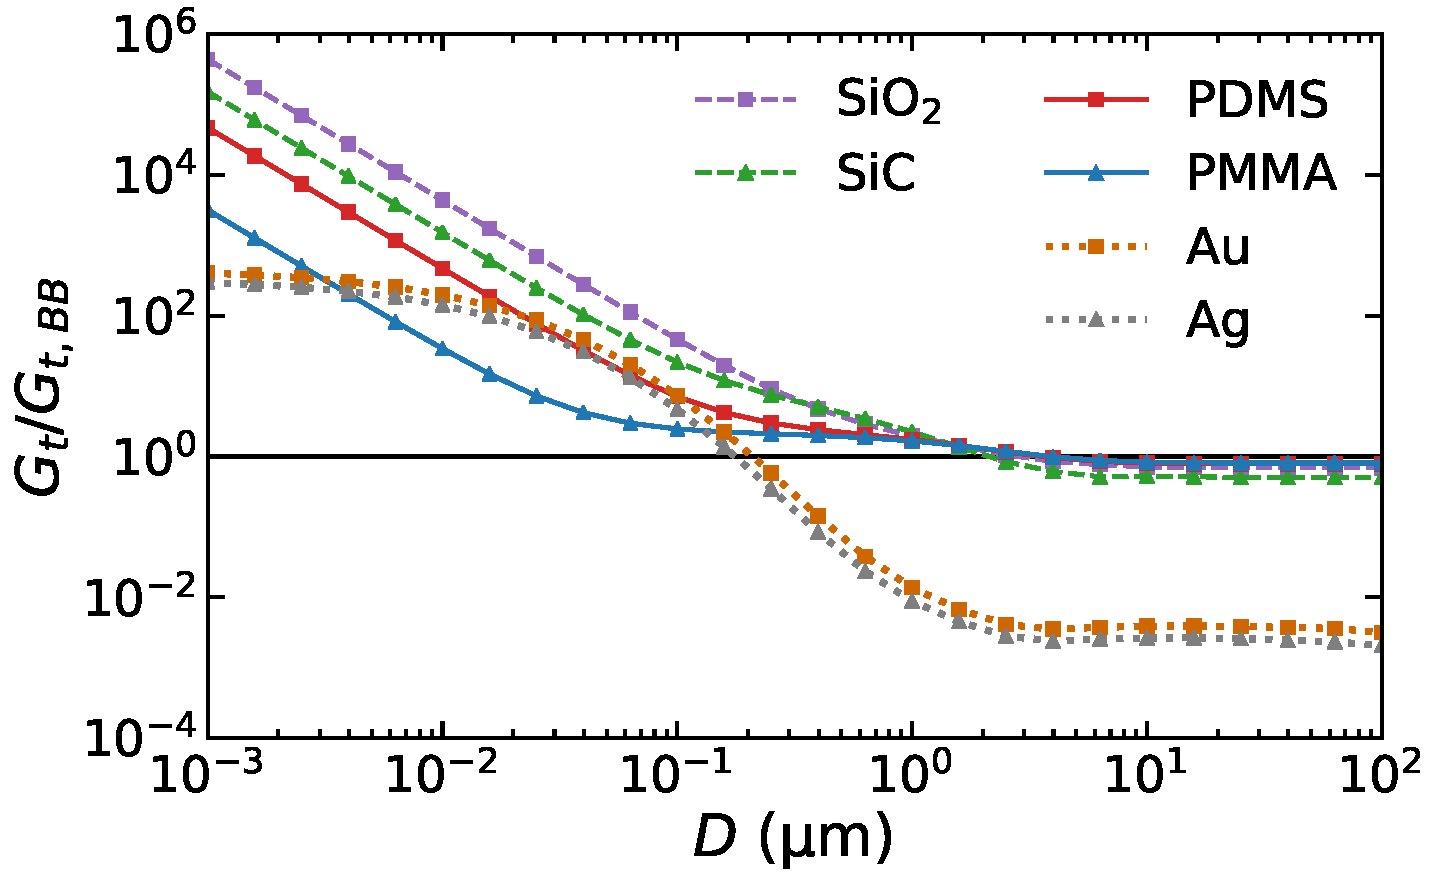
\includegraphics[width=0.8\textwidth]{./Figures/NFRHT_planeplane_total.pdf}
\caption{\label{fig:PlanePlane_total}Total conductance between two semi-infinite planar bodies. The conductance is computed for polar dielectrics (SiO$_{2}$ and SiC), polymers (PDMS and PMMA), and metals (Au and Ag). The conductance is normalized in the plot by that of two blackbodies ($G_{t,BB}/A = 6.12$ \si{\watt\per\square\meter\per\kelvin} where $A$ is the surface area). The solid black line lies at an ordinate of 1 (blackbody behavior) for all values of abscissa.}
\end{figure}

Figure \ref{fig:PlanePlane_total} shows the spectral conductance at a fixed separation distance of 0.1 \si{\micro\meter}. This distance was chosen because it lies safely within the near-field.  Dielectric materials show mostly level behavior (indicating a graybody approximation is valid at those wavelengths), with some peaks seemingly superimposed on top. The peaks correspond to the locations of resonances of the dielectric function of each material.\cite{Spitzer1959, Srinivasan2016, Tsuda2018} The three largest peaks present (two large peaks for silicon dioxide at 8.5 \si{\micro\meter} and 20 \si{\micro\meter} and one large peak at 10.5 \si{\micro\meter} for silicon carbide) correspond to SPhP modes. The other peaks occur due to optical resonances that do not qualify as SPhP modes. Those peaks, such as the numerous peaks in the spectra of PDMS and PMMA, tend to be much smaller. Unsurprisingly, the metals act unlike any other material and do not conform to the shape of a blackbody distribution.

\begin{figure}
\centering
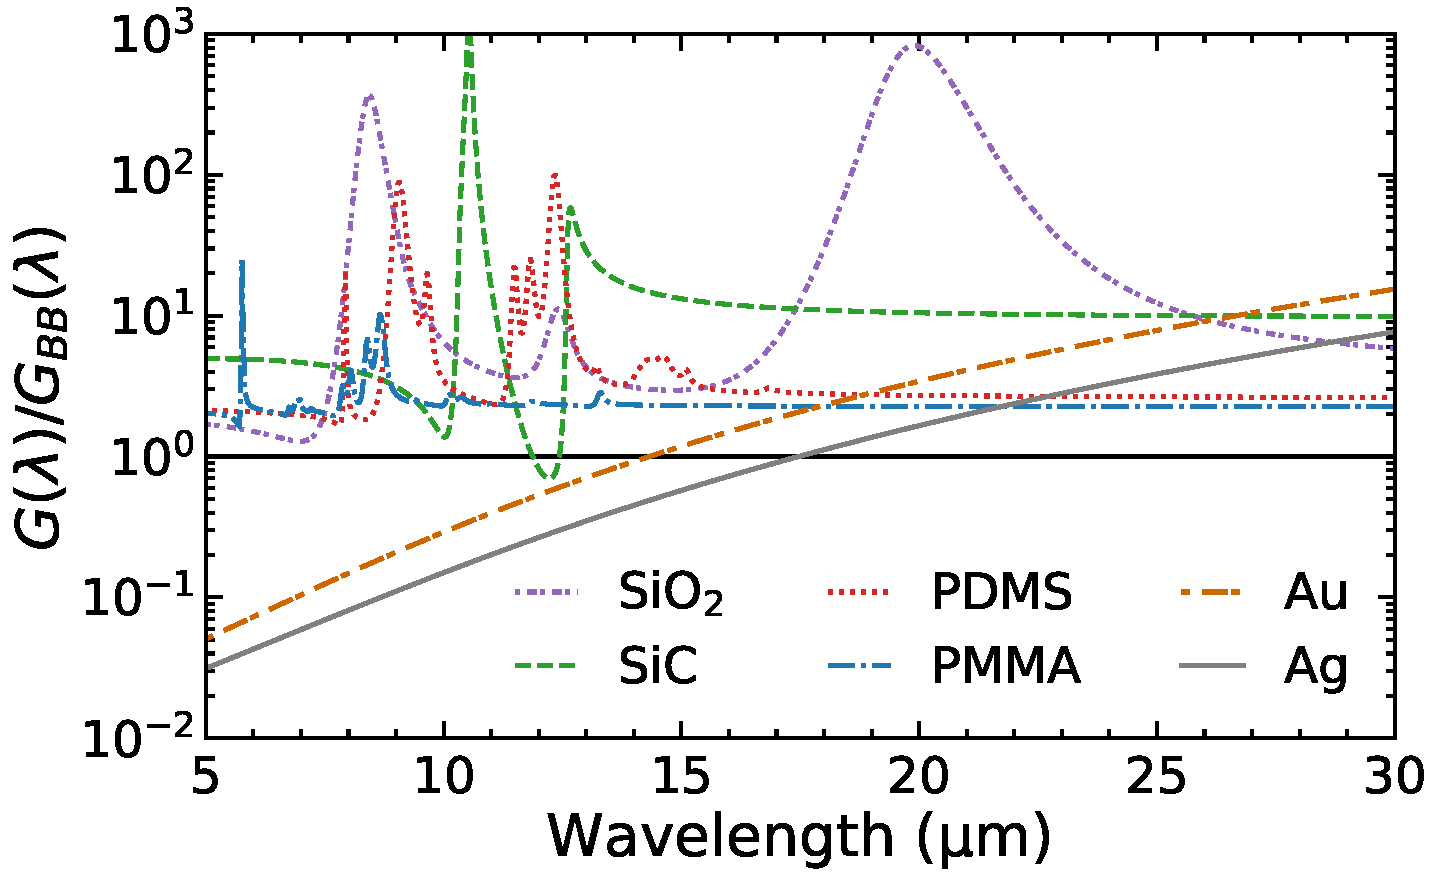
\includegraphics[width=0.8\textwidth]{./Figures/NFRHT_planeplane_spectral_fixedgap.pdf}
\caption{\label{fig:PlanePlane_spectral_onegap}Spectral conductance between two semi-infinite planar bodies with a separation distance of 0.1 \si{\micro\meter}. The conductance is computed for polar dielectrics (SiO$_{2}$ and SiC), polymers (PDMS and PMMA), and metals (Au and Ag). The conductance is normalized in the plot by that of two blackbodies. The solid black line lies at an ordinate of 1 (blackbody behavior) for all values of abscissa.}
\end{figure}

Reviewing NFRHT between planar surfaces was meant to demonstrate some of the common features of NFRHT in the simplest test-case. Many of these characteristics will appear again when examining NFRHT between spheres. The details of that configuration are presented in Chapters \ref{ch:model} and \ref{ch:results}.